
\begin{dialog}{施德鲁,人设计的玩具\note{本篇对话采自特里·维诺格拉德;“语言理解的过程性模型”,载尚克与科尔比[R.Schank;K.Colby]编《思维与语言的计算机模型》,第155--166页。本书作者只改动了两个角色的名字。为了与汉语的语法相符合,译文中有修改。}}

\begin{quote}
有一天,伊她·娥英女士漫步到麻省理工学院人工智能实验室,碰上了才气横溢的青年计算机程序施德鲁。施德鲁正急着找人来试验试验新近开发出来的一个人——“格拉德·维维诺诺博士”。施德鲁向伊她说明:这位格拉德·维维诺诺博士在他的专业领域里是颇为聪明的,他的专业是分析关于一种“玩具世界”的对话,而这种“玩具世界”由各种不同形状、不同大小、不同颜色的积木组成。这些积木摆在一张桌子上,可以捡起来,挪到别的位置。伊她女士一听就着了迷,立刻在施德鲁的鍵盘上噼哩啪啦地打起字来。格拉德·维维诺诺博士答应站在她身后随时提供一些说明。
\end{quote}

\begin{figure}
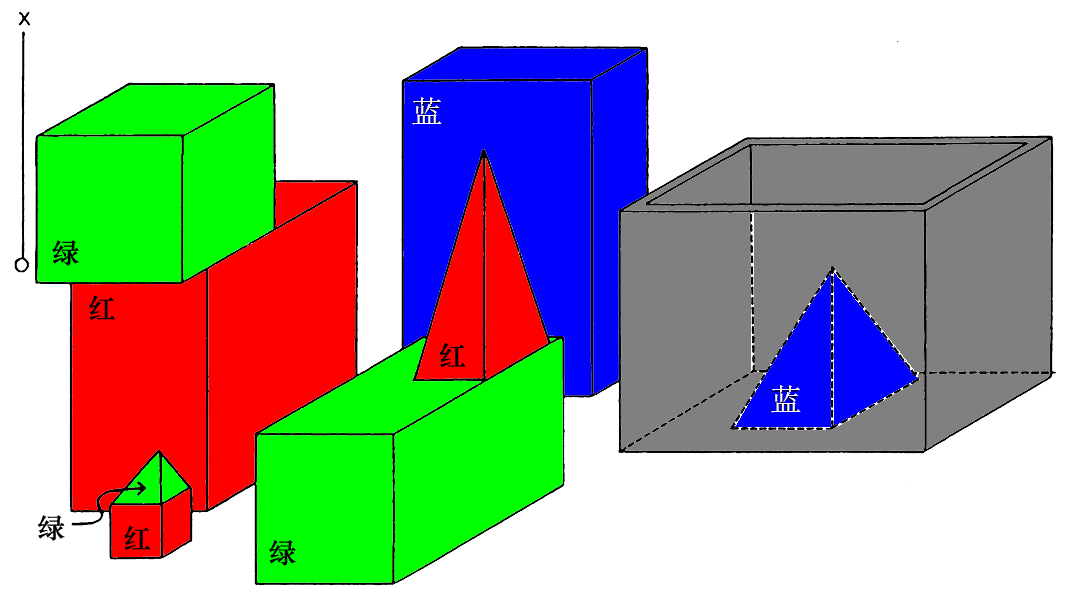
\includegraphics{img_110.png}
\caption[与施德鲁对话开始时的情景。]
  {“拣起一个大红方块。”[选自特里·维诺格拉德,《理解自然语言》,第8页。]}
\end{figure}

\begin{enumerate}[labelindent=0pt,label=\arabic*.,format=\bfseries,widest*=44]

\setnamewidth{\ccwd}

\item \begin{dialogue}
\item[伊她·娥英]拣起一个大红方块。\lnote{[参见\fig{110}]}
\item[施德鲁]行。
\item[格拉德·维维诺诺博士]施德鲁执行命令时候照例回答:“行!”。为拣起这个红方块,须先找出一个地方,以便移开上面的绿方块。
\end{dialogue}

\item \begin{dialogue}
\item[伊她·娥英]抓住那个方锥。
\item[施德鲁]我不明白你指的是哪个方锥。
\item[格拉德·维维诺诺博士]屏幕上有三个方锥,施德鲁懂得“那个”所指的是说话人心目中的一个对象。
\end{dialogue}

\item \begin{dialogue}
\item[伊她·娥英]找一块比你手里的那块大点的积木,把它搁到盒子里。\lnote{[参见\fig{111}]}

\begin{figure}
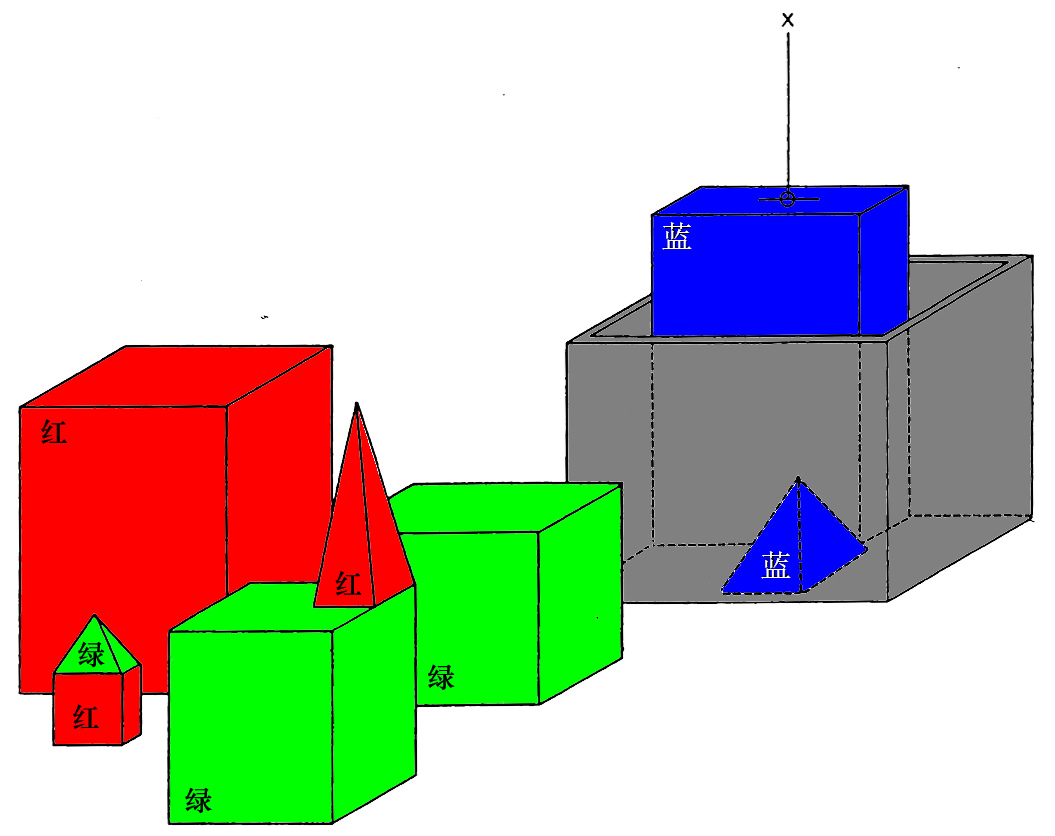
\includegraphics{img_111.png}
\caption[与施德鲁对话一段时间后的情景。]
  {“找一块比你手里的那块大点的积木,把它搁到盒子里。”[选自维诺格拉德,《理解自然语言》,第9页。]}
\end{figure}

\item[格拉德·维维诺诺博士]施德鲁先要弄清“那块”、“它”各指什么,还要推定“手里”有什么。
\item[施德鲁]“它”指大点的那块积木。
\item[格拉德·维维诺诺博士]施德鲁能用启发规则确定“它”所指的是“手里的那块”还是“找”出来的那块。
\item[施德鲁]行。
\item[格拉德·维维诺诺博士]施德鲁须先放下红方块,才能拣起蓝方块。
\end{dialogue}

\item \begin{dialogue}
\item[伊她·娥英]盒子里都有什么?
\item[施德鲁]蓝方锥和蓝方块。
\end{dialogue}

\item \begin{dialogue}
\item[伊她·娥英]方锥下边是什么?
\item[格拉德·维维诺诺博士]以前说“方锥”时,施德鲁说“我不明白你说的是哪个方锥”。现在,他认为你所说的就是刚才谈及的那个方锥。
\item[施德鲁]盒子底。
\end{dialogue}

\item \begin{dialogue}
\item[伊她·娥英]有几个方块没在盒子里?
\item[格拉德·维维诺诺博士]施德鲁能掌握各种不同的否定词语的含义,例如“没”,“不”等等。
\item[施德鲁]四个。
\end{dialogue}

\item \begin{dialogue}
\item[伊她·娥英]这四个方块里有没有比我刚说让你拣起的那块大的?
\item[格拉德·维维诺诺博士]“这四个方块”指上一问题中谈及的方块;“比……大的”也应指方块。名词短语中可能含有复杂的数量词,如“至少一块”、“三块以上”、“恰好七块”等。为确定“我刚才让你拣起的那块”,需要用到已发生事件的记录。此外,“我刚才说让你拣起的”和“那块”的句法关系是间接的。施德鲁的句法分析程序能以一种具有普遍性的方式处置这种复杂的句法关系。
\item[施德鲁]有,就是那个红方块。
\end{dialogue}

\item \begin{dialogue}
\item[伊她·娥英]它下边有东西吗?
\item[施德鲁]有,桌面。
\item[格拉德·维维诺诺博士]施德鲁用启发规则以确定对于人有关的信息,即使问题中并未明确提出要求。
\end{dialogue}

\item \begin{dialogue}
\item[伊她·娥英]桌子能不能拣木块?
\item[施德鲁]不能。
\item[格拉德·维维诺诺博士]只有动物才能拣东西,而桌子不是动物。施德鲁的语义规则具备这些知识。
\end{dialogue}

\item \begin{dialogue}
\item[伊她·娥英]方锥能不能搁在方块上?
\item[施德鲁]能。
\item[格拉德·维维诺诺博士]施德鲁的推理系统发现了一个例证,所以他知道这是可能的。
\end{dialogue}

\item \begin{dialogue}
\item[伊她·娥英]方锥上能不能搁方块?
\item[施德鲁]不知道。
\item[格拉德·维维诺诺博士]这个问题本身是有意义的,但是在屏幕上并没有出现例证。施德鲁无法看到他自己的程序里的细节,尽管他的能力终究是由这些细节所确定的。
\end{dialogue}

\item \begin{dialogue}
\item[伊她·娥英]把两个方锥摞起来。
\item[施德鲁]我摞不起来。
\item[格拉德·维维诺诺博士]施德鲁尝试这样做,但失败了。
\end{dialogue}

\item \begin{dialogue}
\item[伊她·娥英]蓝方锥是松木的。
\item[施德鲁]明白了。
\item[格拉德·维维诺诺博士]施德鲁知道对象的颜色、形状,大小和位置。质料则是对象的未知性质。告诉它以后,它就记录在数据库中。
\end{dialogue}

\item \begin{dialogue}
\item[伊她·娥英]除了红的木块和方锥下边的木块以外,都是松木的。
\item[施德鲁]明白了。
\item[格拉德·维维诺诺博士]施德鲁对这句话的理解,导致它建立一个新的推理过程,以确定某个木块是否是松木的。
\end{dialogue}

\item \begin{dialogue}
\item[伊她·娥英]盒子是不是松木的?
\item[施德鲁]不是。
\item[格拉德·维维诺诺博士]盒子中有个方锥,盒子是方锥下面的东西。
\end{dialogue}

\item \begin{dialogue}
\item[伊她·娥英]盒子里有松木的东西吗?
\item[施德鲁]有两个:蓝方块和蓝方锥。
\end{dialogue}

\item \begin{dialogue}
\item[伊她·娥英]你把两个红方块跟一个绿色的方块或是方锥摞成一摞,好吗?\lnote{[参见\fig{112}]}

\begin{figure}
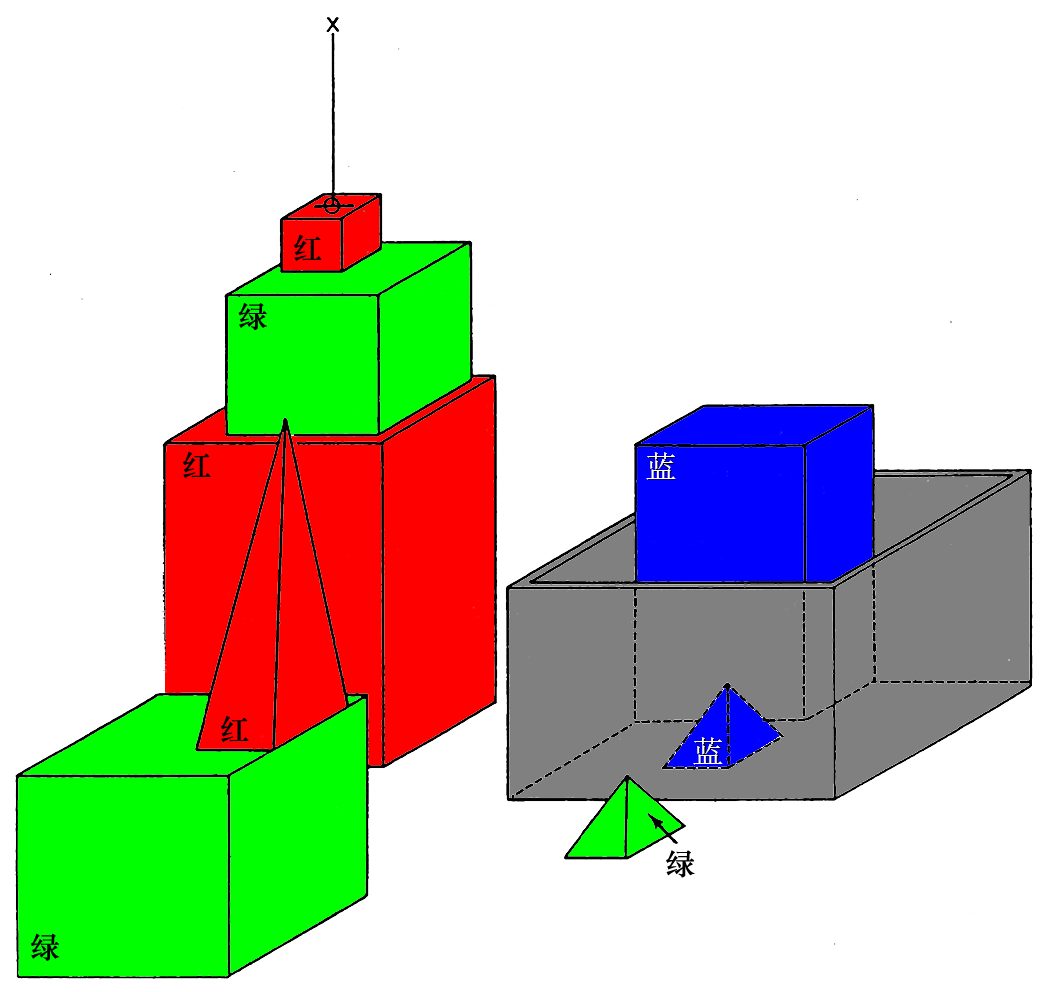
\includegraphics{img_112.png}
\caption[与施德鲁对话最后时的情景。]
  {“你把两个红方块跟一个绿色的方块或是方锥摞成一摞,好吗?”[选自维诺格拉德,《理解自然语言》,第12页。]}
\end{figure}

\item[施德鲁]行。
\item[格拉德·维维诺诺博士]对“跟”、“或是”这类逻辑联词的处理同时考虑到了语法和语义。一个命令即使形式上是一个问题也会被执行。这个命令执行过程如下:把一个绿方块放在大红方块上(他选中的是上面没有东西的绿方块),把小红方块上面的小方锥移开,再把小红方块摞到绿方块上面。
\end{dialogue}

\item \begin{dialogue}
\item[伊她·娥英]哪个方块是放在桌面上的?
\item[施德鲁]红方锥底下的大绿方块。
\item[格拉德·维维诺诺博士]一般说来回答“大绿方块”已经满意了,但就这个问题而言,最好把它限定得清楚一些。
\end{dialogue}

\item \begin{dialogue}
\item[伊她·娥英]有没有放在方锥后边的大块积木?
\item[施德鲁]有三块:一个大红方块,一个大绿方块,一个大蓝方块。
\end{dialogue}

\item \begin{dialogue}
\item[伊她·娥英]往那个上面放着方锥的绿方块上再搁上一个小方块。
\item[施德鲁]行。
\end{dialogue}

\item \begin{dialogue}
\item[伊她·娥英]把最小的方锥搁到它上面。
\item[格拉德·维维诺诺博士]施德鲁先要比较所有方锥的大小,再采取行动。
\item[施德鲁]行。
\end{dialogue}

\item \begin{dialogue}
\item[伊她·娥英]有多少东西是放在绿方块上面的?
\item[施德鲁]你说“放在绿方块上面”,我不明白这个“上面”指什么意思。你是指:
  \begin{enumerate}[label=(\arabic*)]
  \item 与它的表面接触,还是
  \item 在它上方的任何地方?
  \end{enumerate}
\item[格拉德·维维诺诺博士]前面那一句话里,“上面”的解释未发生困难,是因为从上下文中可以澄清它的含义。在这一句话里,解释歧义的启发规则无法做出清楚的定义。施德鲁只好向你要求进一步的信息。类似的问题在解释“它”、“那些”等词的时候也可能遇到。
\end{dialogue}

\item \begin{dialogue}
\item[伊她·娥英]你把绿方锥放在小方块上面以前动过哪个方锥没有?
\item[施德鲁]动过绿的。
\item[格拉德·维维诺诺博士]施德鲁能从它的记忆中找出现在说的是什么事件,并能把它和别的事件前后联系起来。对于本句的分析涉及像“没有”这样的词的种种不同用法。
\end{dialogue}

\item \begin{dialogue}
\item[伊她·娥英]你是什么时候动的它?
\item[施德鲁]我把两个红方块跟一个绿方块摞起来的时候。
\item[格拉德·维维诺诺博士]时间可以用当时所作的工作来描述。
\end{dialogue}

\item \begin{dialogue}
\item[伊她·娥英]为什么要动它?
\item[格拉德·维维诺诺博士]施德鲁记得前一句对话,因此能理解这类问题。
\item[施德鲁]把它拿到一边去。
\item[格拉德·维维诺诺博士]施德鲁能从原有的子目标树找出其工作的每一步骤的目的。
\end{dialogue}

\item \begin{dialogue}
\item[伊她·娥英]这又是为什么?
\item[施德鲁]好把它下边的红方块抓起来。
\item[格拉德·维维诺诺博士]“这”指的是前一答句中的动作。
\end{dialogue}

\item \begin{dialogue}
\item[伊她·娥英]为什么要抓那个红方块?
\item[格拉德·维维诺诺博士]“那个”指的是前一句里所说的红方块。
\item[施德鲁]好把它放在一个大绿方块上。
\end{dialogue}

\item \begin{dialogue}
\item[伊她·娥英]这又是为什么?
\item[施德鲁]好把两个红方块和一个大绿方块摞起来。
\end{dialogue}

\item \begin{dialogue}
\item[伊她·娥英]这又是为什么?
\item[施德鲁]你让我这样做的。
\item[格拉德·维维诺诺博士]施德鲁记得他做了什么,而不是对它的要求的原话。
\end{dialogue}

\item \begin{dialogue}
\item[伊她·娥英]这件事你是怎样做的?
\item[格拉德·维维诺诺博士]“这件事”指的是前一问句里所说的事。
\item[施德鲁]把一个大红方块放在桌上,松手,再把一个红方块放在绿方块上,松手。
\item[格拉德·维维诺诺博士]本句描述了为实现一个目标所建立的最高层子目标。
\end{dialogue}

\item \begin{dialogue}
\item[伊她·娥英]你干这些事的时候动了多少木块?
\item[格拉德·维维诺诺博士]“干这些事的时候”指的是一段时间。
\item[施德鲁]四块。
\end{dialogue}

\item \begin{dialogue}
\item[伊她·娥英]你抓起小红方块以前,它上面有什么?
\item[施德鲁]绿方锥。
\item[格拉德·维维诺诺博士]回顾以往的动作可以推算过去的场面。
\end{dialogue}

\item \begin{dialogue}
\item[伊她·娥英]那时候盒子左边有五块积木。
\item[格拉德·维维诺诺博士]“那时候”是指上一句所说的时间。
\item[施德鲁]没有,只有四块:两个红方块跟两个绿方块。
\item[格拉德·维维诺诺博士]前边说到质料,施德鲁马上接受了。但他知道他具有关于木块位置的全部信息,所以他要与它的知识进行核对,并表示同意与否。
\end{dialogue}

\item \begin{dialogue}
\item[伊她·娥英]把蓝方锥搁在盒子里的蓝方块上头有问题吗?
\item[格拉德·维维诺诺博士]这句话句法上是有歧义的,因为它可以分析为“把蓝方锥搁在盒子里”的“蓝方块”上头有某种东西与否。施德鲁会排除这种句法歧义。
\item[施德鲁]没问题。
\end{dialogue}

\item \begin{dialogue}
\item[伊她·娥英]搁上去吧。
\item[施德鲁]行。
\end{dialogue}

\item \begin{dialogue}
\item[伊她·娥英]一个塔……
\item[施德鲁]对不起,我不明白什么叫“塔”。
\item[格拉德·维维诺诺博士]施德鲁读到一个不知道的字,就会打断你的话。
\end{dialogue}

\item \begin{dialogue}
\item[伊她·娥英]“塔”是用两个绿方块和一个方锥做成的。
\item[格拉德·维维诺诺博士]你用了引号,施德鲁知道你在解释一个生词,于是就用适当的形式把这个词放在词汇表里。
\item[施德鲁]明白了。
\end{dialogue}

\item \begin{dialogue}
\item[伊她·娥英]现在有没有塔?
\item[施德鲁]没有。
\item[格拉德·维维诺诺博士]新定义可以用于辨认塔。
\end{dialogue}

\item \begin{dialogue}
\item[伊她·娥英]你做一个吧。
\item[施德鲁]行。
\item[格拉德·维维诺诺博士]新定义也可以用于判定建造的计划。这里“一个”指的就是“塔”。于是施德鲁就可以出如下的计划:把两个大绿方块摞起来,并把红方锥放在上面。
\end{dialogue}

\item \begin{dialogue}
\item[伊她·娥英]把最大的那个木块叫做“大胖子”。
\item[施德鲁]行。
\item[格拉德·维维诺诺博士]可以给木块取名字。
\end{dialogue}

\item \begin{dialogue}
\item[伊她·娥英]你动过大胖子吗?
\item[施德鲁]动过。
\item[格拉德·维维诺诺博士]“动过”当然是指从对话开始以来。
\end{dialogue}

\item \begin{dialogue}
\item[伊她·娥英]你怎么把它丢了?
\item[施德鲁]我想你说的“它”指的是大胖子。但是我不能解释一件没有发生过的事情。
\item[格拉德·维维诺诺博士]施德鲁从它的记录中查不到丢木块的事件。它有专门的程序对付这类“别有用心”的问题。
\end{dialogue}

\item \begin{dialogue}
\item[伊她·娥英]红方锥的右边有什么?
\item[施德鲁]有四样东西:盒子,小红方块,蓝方锥和叫做大胖子的那块积木。
\item[格拉德·维维诺诺博士]所取的名字也可以用于指称事物。
\end{dialogue}

\item \begin{dialogue}
\item[伊她·娥英]谢谢你!
\item[施德鲁]不客气!
\item[格拉德·维维诺诺博士]施德鲁的语法知识实际上是一个程序,这个程序使他能处理惯用语。
\end{dialogue}

\end{enumerate}

\end{dialog}
